\subsection{Gihub}
\begin{frame}
    \frametitle{Github --- Social Coding \hfill{} LuXeria}
    \framesubtitle{Was soll das sein?}
    \begin{columns}
        \begin{column}{5cm}
            \begin{figure}
                
\includegraphics[scale=0.15]{github_logo.eps}
                \caption{Github -- Logo}
            \end{figure}
            \begin{figure}
                
\includegraphics[scale=0.08]{github_network.jpg}
                \caption{Soziales Netzwerk}
            \end{figure}
        \end{column}
        \begin{column}{5cm}
            \begin{block}{Was ist Github?}
                \begin{itemize}
                    \item Host für Repositories
                    \item Private \& Enterprise
                    \item Nr. 2 unter Hosts
                \end{itemize}
            \end{block}
            \begin{block}{Was ist speziell?}
                \begin{itemize}
                    \item User im Zentrum
                    \item Projektverwaltung
                    \item Git-Anbindung
                    \item Simpel \& stabil
                \end{itemize}
            \end{block}
        \end{column}
    \end{columns}
\end{frame}

\begin{frame}
    \frametitle{Github --- Überblick \hfill{} LuXeria}
    \framesubtitle{Einige Daten}
    \begin{columns}
        \begin{column}{5cm}
            \begin{block}{Berühmte Repos}
                \begin{itemize}
                    \item Erlang
                    \item Linux Mint
                    \item jQuery
                    \item Perl
                    \item PHP
                    \item Ruby (Iron, Rails...)
                    \item Python
                    \item Twitter
                \end{itemize}
            \end{block}
        \end{column}
        \begin{column}{5cm}
            \begin{block}{Nutzung und Service}
                \begin{itemize}
                    \item +3'000'000 User
                    \item +4'000'000 Repos
                    \item Most Popular Host
                    \item offene API
                    \item Webhosting (static)
                    \item Support \& Training
                \end{itemize}
            \end{block}
        \end{column}
    \end{columns}
\end{frame}

\begin{frame}
    \frametitle{Github --- User \hfill{} LuXeria}
    \framesubtitle{Über User und ihre Repos}
    \begin{columns}
        \begin{column}{5cm}
            \begin{figure}
            
\includegraphics[scale=0.15]{github_social.jpg}
            \caption{Soziales Netzwerk}
            \end{figure}
        \end{column}
        \begin{column}{5cm}
            \begin{block}{User in Github}
                \begin{itemize}
                    \item haben eine Profilseite
                    \item haben eigene Repos
                    \item verfolgen User \& Repos
                    \item Chatten über Code
                    \item feed-, follow-,  starr- \& forken
                    \item beobachten Projekt-Analysen
                    \item führen Repo Wikis
                    \item setzten Webpages auf
                \end{itemize}
            \end{block}
        \end{column}
    \end{columns}
\end{frame}

\begin{frame}
    \frametitle{Github --- Issues \hfill{} LuXeria}
    \framesubtitle{Über Repos und Angelegenheiten}
    \begin{figure}
        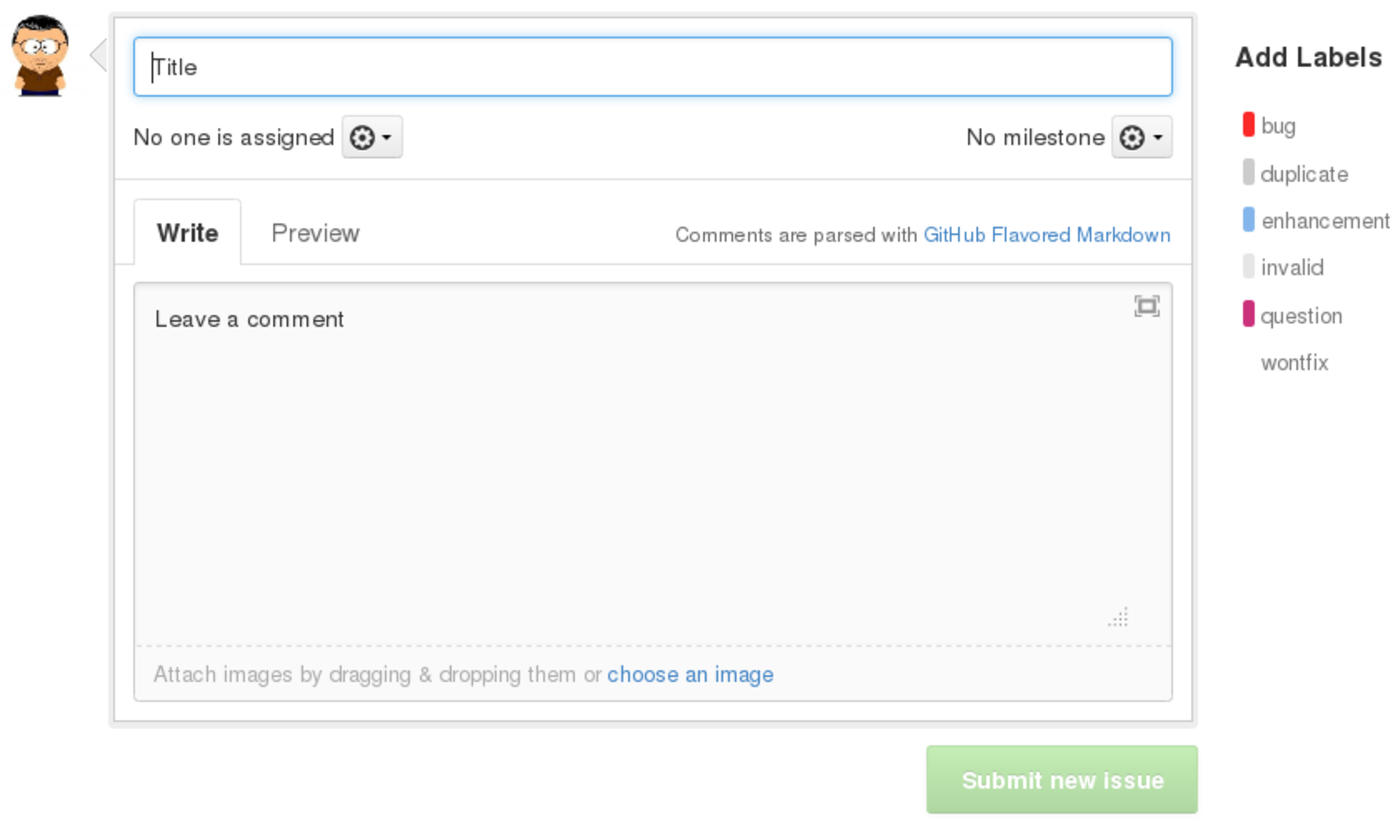
\includegraphics[width=0.8\textwidth]{github_issue.pdf}
        \caption{Issue erstellen}
    \end{figure}
\end{frame}

\begin{frame}
    \frametitle{Github --- Meilenstein \hfill{} LuXeria}
    \framesubtitle{Projektmanagement ist auch beim Code wichtig!}
    \begin{figure}
        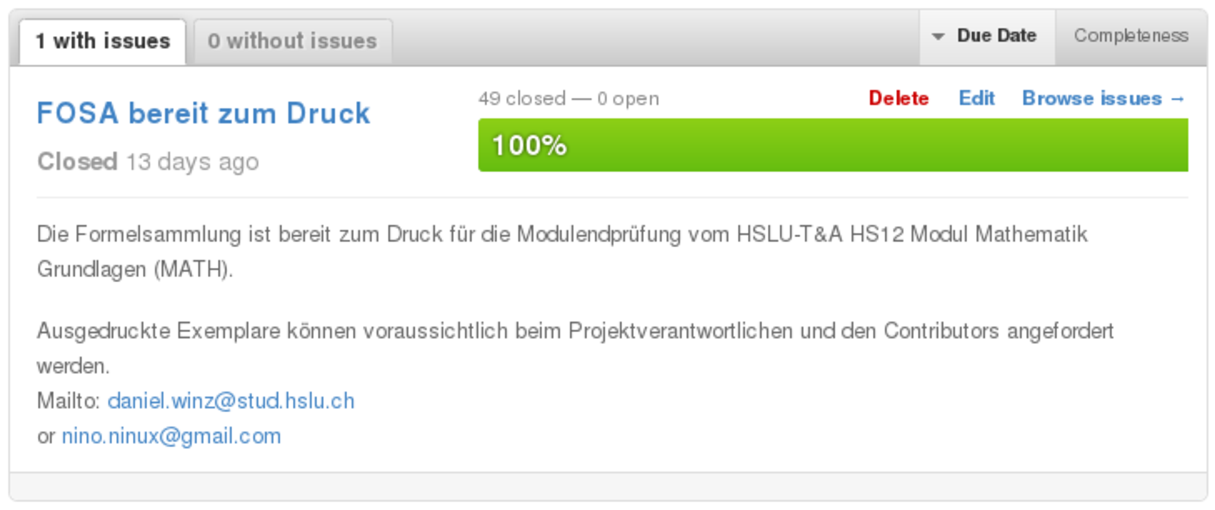
\includegraphics[width=0.9\textwidth]{github_milestone.pdf}
        \caption{Meilenstein}
    \end{figure}
\end{frame}

\begin{frame}
    \frametitle{Github --- Graphs \hfill{} LuXeria}
    \framesubtitle{Contributor Graph -- Wer ist dabei und wer macht wieviel?}
    \begin{figure}
        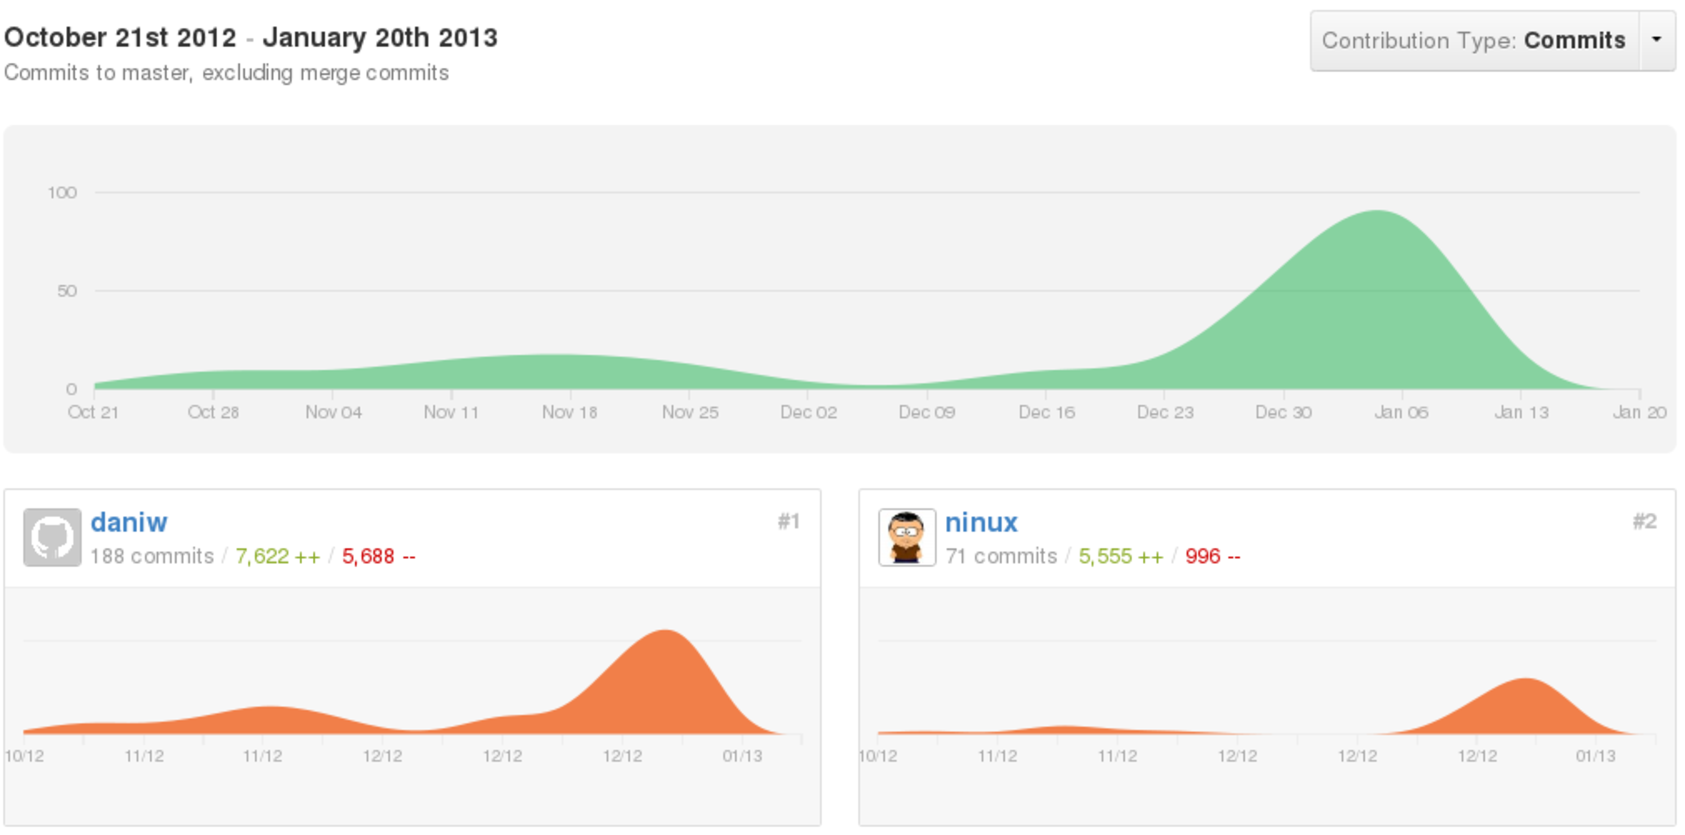
\includegraphics[width=0.9\textwidth]{github_contributors.pdf}
        \caption{Teinnehmer}
    \end{figure}
\end{frame}

\begin{frame}
    \frametitle{Github --- Graphs \hfill{} LuXeria}
    \framesubtitle{Commits -- Wie aktiv wird am Projekt entwickelt? }
    \begin{figure}
        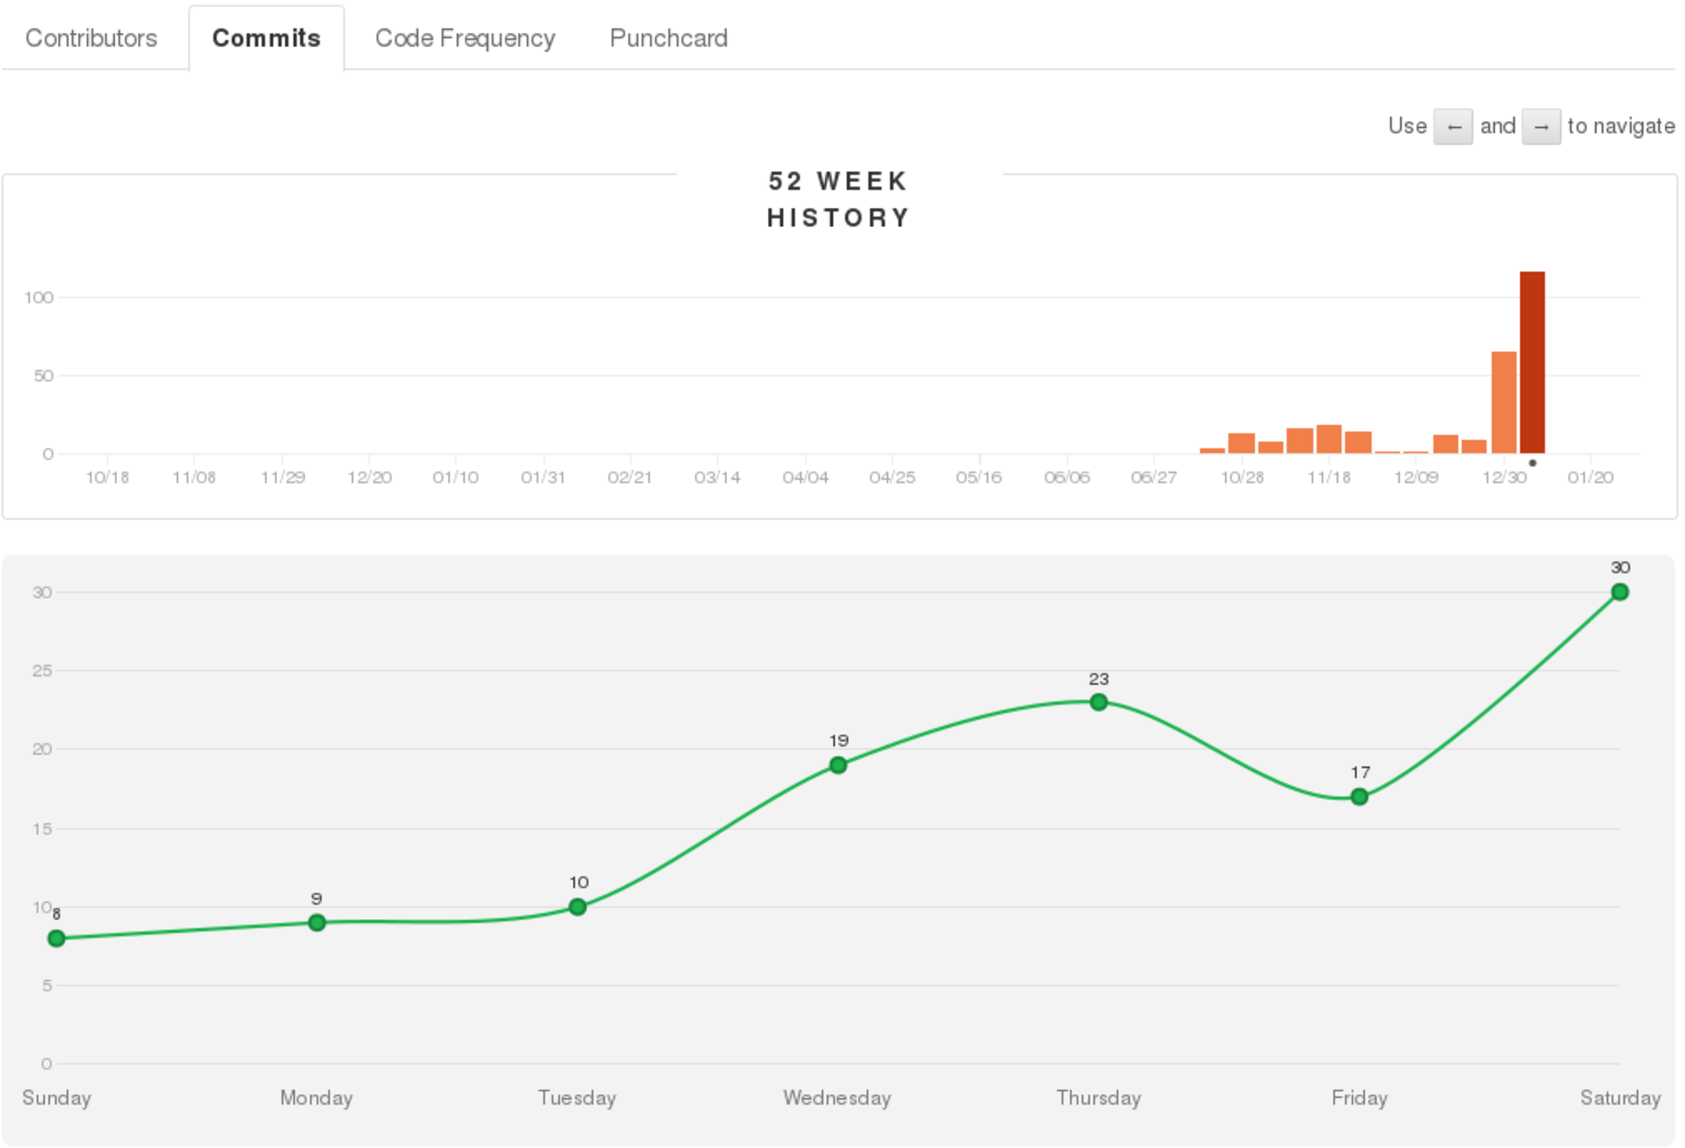
\includegraphics[width=0.8\textwidth]{github_commits.pdf}
        \caption{Commits}
    \end{figure}
\end{frame}

\begin{frame}
    \frametitle{Github --- Graphs \hfill{} LuXeria}
    \framesubtitle{Punchcard -- Der Wochenspiegel}
        \begin{figure}
            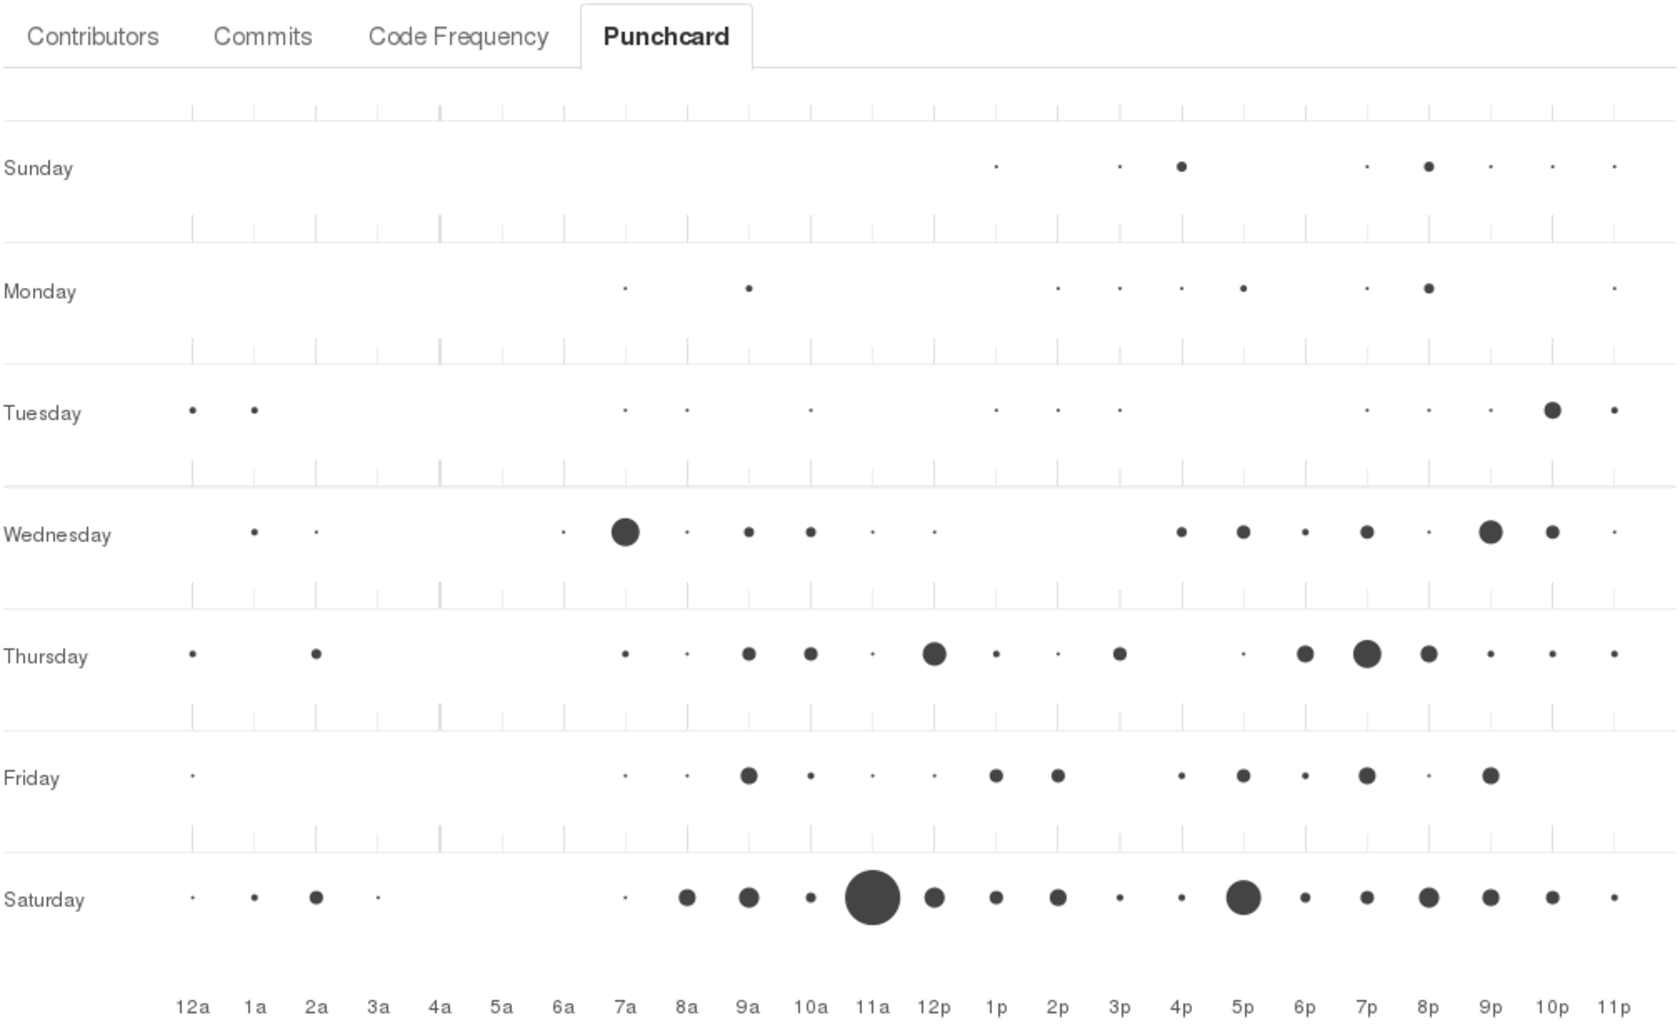
\includegraphics[width=0.8\textwidth]{github_punchcard.pdf}
            \caption{Punchcard}
        \end{figure}
\end{frame}

\begin{frame}
    \frametitle{Github --- Graphs \hfill{} LuXeria}
    \framesubtitle{Network -- Behalte den Flow im Auge!}
        \begin{figure}
            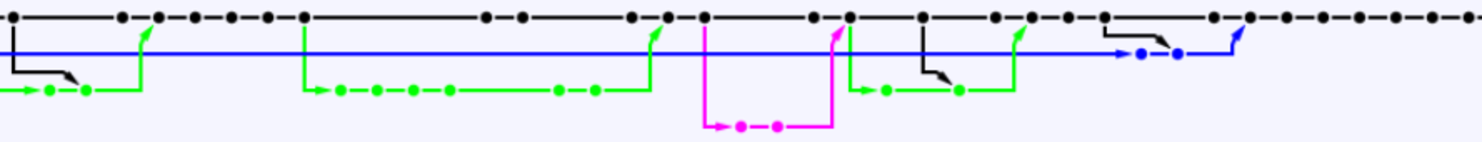
\includegraphics[width=0.9\textwidth]{github_network.pdf}
            \caption{Network}
        \end{figure}
\end{frame}

\begin{frame}
    \frametitle{Github --- Mobile \hfill{} LuXeria}
    \framesubtitle{Github auf Android und iOS}
    \begin{columns}
        \begin{column}{5cm}
            \begin{figure}
                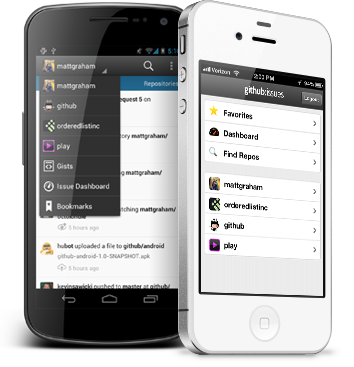
\includegraphics[width=0.6\textwidth]{github_mobile2.png}
                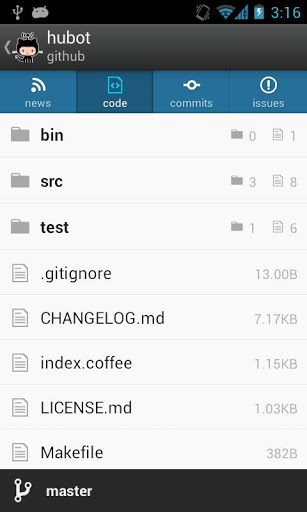
\includegraphics[width=0.38\textwidth]{github_mobile.jpg}
                \caption{Github Unterwegs}
            \end{figure}
        \end{column}
        \begin{column}{5cm}
            \begin{block}{Facebookst du noch oder Githubst du schon?}
                \begin{itemize}
                    \item Gists - tausche snippets
                    \item Issue Dashboard
                    \item Repositories
                    \item Followers
                    \item Following
                    \item Newsfeed
                    \item check Commits
                \end{itemize}
            \end{block}
        \end{column}
    \end{columns}
\end{frame}


